%! TEX program = xelatex
% 排版底版：latexstudio/CUMCMThesis，2026/08/26 v2.9。
% cumcm2026base.cls 为上游类文件，仅改类名；cumcm2026.sty 为上游2026配套样式。
\PassOptionsToPackage{quiet}{xeCJK}
\documentclass[withoutpreface,bwprint]{cumcm2026base}
\usepackage{cumcm2026}
\usepackage[super,numbers,sort&compress]{natbib}
\BeforeBeginEnvironment{tabular}{\zihao{-5}}
% 居中伸缩列采用2026样式提供的Y列。
\newcommand{\placeholder}[1]{\textcolor{gray}{【#1】}}
\renewcommand{\thesection}{\arabic{section}}
\renewcommand{\thesubsection}{\thesection.\arabic{subsection}}
\renewcommand{\thesubsubsection}{\thesubsection.\arabic{subsubsection}}
\makeatletter
\renewcommand{\mcm@cap@keywordsname}{关键词}
\makeatother
\hypersetup{colorlinks=true,linkcolor=black,citecolor=black,urlcolor=black}
\graphicspath{{figures/}{./}}
\title{基于几何证书与主动测量的多干扰源定位清除模型}
\tihao{B}
\yearinput{2026}
\monthinput{9}
\dayinput{10}
\begin{document}
\maketitle
\begin{abstract}
本文研究移动机器人在部分可观测环境中对多个无线电干扰源进行主动搜索、定位与清除的问题。围绕测向误差、未知接收半径、多频道切换以及定向发射等因素，建立由几何定位、信念更新和路径决策组成的统一模型。

\textbf{针对问题一，}将每次测向观测表示为带角度误差的扇形可行域，通过半平面裁剪求取多次观测的交集，并利用最远点对和最小包围圆刻画定位精度与清除可行性。\placeholder{补充最终精度、误差或判定阈值。}

\textbf{针对问题二，}建立以单位虚拟时间信息增益为指标的下一最佳观测点模型，兼顾交会角、移动距离和失去信号风险。\placeholder{补充第二检测点坐标及相较基线的提升。}

\textbf{针对问题三，}把多源搜索抽象为部分可观测决策过程，以粒子集合维护各频道的位置后验，结合候选动作生成与有限步信念空间规划，联合优化测量、移动、清除和频道切换。\placeholder{补充正式模拟器中的清除率和平均耗时。}

\textbf{针对问题四，}进一步引入未知发射方向与无信号观测的多义性，通过定向源状态扩维、域随机化和覆盖兜底策略提高模型稳健性。\placeholder{补充问题四的核心数值结论。}

最后，从定位误差、策略稳定性和计算效率三个方面检验模型。结果表明，\placeholder{用一句话填写最有竞争力、且已经由程序复现的结论。}

\keywords{主动定位\quad 信念空间规划\quad 部分可观测决策过程\quad 信息增益\quad 路径优化}
\end{abstract}

\section{问题背景和分析}

\subsection{问题背景}
无线电干扰源的搜索与清除同时包含主动感知和路径规划：机器人需要移动到合适位置获取方向信息，又要控制移动、检测、频道切换和清除产生的时间成本。由于目标数量、位置、有效接收半径和发射方向均不可直接观测，单次测量不足以确定目标；同时，错误退出会遗漏未发现频道，因此策略既要追求效率，也要给出发现、清除和退出的可靠依据。

本文将四问组织为一条递进技术路线：问题一构造有界误差下的定位与清除证书，问题二选择兼顾观测可靠性和定位质量的第二检测点，问题三建立全向多源的完备搜索骨架和频道状态机，问题四把覆盖保证推广到含未知发射方向的定向源场景。

\subsection{问题一分析}
每次测向形成一个朝前的角度扇形。多个扇形相交后得到干扰源可行域。问题一除要求计算区域直径外，还需判断由最远点对构造的直径圆能否覆盖该区域；为此必须区分“区域直径”和“覆盖区域所需的最小半径”。

\subsection{问题二分析}
第二检测点既要与已有测向方向形成良好交会角，又要避免因未知接收半径而失去信号。本文先限制候选点位于保证接收区域，再比较其移动时间和最坏后验定位半径。

\subsection{问题三分析}
全向源的无信号观测能够排除检测点周围半径 $1000\,\mathrm{m}$ 的区域。因而可以设计覆盖整个目标圆的检测点集合，既用于发现存在的频道，也用于证明其余频道不存在；在此基础上把搜索、顺路补测和安全清除交织执行。

\subsection{问题四分析}
定向源使无信号同时可能表示距离过远或位于发射方向背面，问题三的圆盘排除不再成立。需要构造同时满足距离覆盖和方向覆盖的检测点布局，并仅用正观测更新位置角域。

\section{问题分析}

\subsection{总体思路}
四问的共同难点是：隐藏状态不能直接获取，观测只能逐步缩小可行集，而清除和退出又必须具有可核验的保证。因此，本文将决策分为两层：几何安全层保留所有满足观测的可能状态，并签发接收、发现、清除和退出证书；效率层只在证书允许的动作中优化观测位置和执行顺序。

问题一提供定位与清除的几何内核，问题二回答“下一次在哪里测”，问题三和问题四分别为全向源和定向源建立连续区域的发现保证。每获得一次观测，程序先更新频道可行域，再判断是否已可安全清除、是否需要补充观测，以及未知频道是否已完成覆盖审计。各问的模型衔接见\cref{tab:roadmap}。

\begin{table}[H]
  \centering
  \caption{四个问题的模型衔接与可核验输出}
  \label{tab:roadmap}
  \begin{tabularx}{\textwidth}{cLLLL}
    \toprule
    问题 & 主要输入 & 核心不确定性 & 建模方法 & 可核验输出 \\
    \midrule
    一 & 多点示向度 & 角度误差有界 & 半平面交、直径与最小包围圆 & 定位区域与安全清除证书 \\
    二 & 首次正观测 & 接收半径未知 & 保证接收约束下的主动选点 & 第二检测点与后验风险估计 \\
    三 & 多频道全向源 & 源数未知 & 七站圆盘覆盖与频道状态机 & 发现或不存在证书、清除路线 \\
    四 & 多频道定向源 & 发射方向未知 & 等边三角网格与正观测更新 & 与方向无关的连续域发现证书 \\
    \bottomrule
  \end{tabularx}
\end{table}

\subsection{问题一分析}
一次示向只限定方向而不给出距离，且误差只有确定上下界。因此不引入未知的概率分布，而将每次观测写成包含真实位置的前向角域，通过集合求交递推缩小可行域\cite{combettes1993}。定位区域为凸集时，其最远点对可由旋转卡壳计算\cite{toussaint1983}；但最远点对只回答直径问题，清除可行性仍需由最小包围圆判定。所以本问的求解链为“角域交一直径一覆盖圆”，并对空集、无界、线段等退化情形单独处理。

\subsection{问题二分析}
观测者的运动会改变仅测向定位的可观性，选点需在交会角改善与移动代价之间权衡\cite{hammel1989}。本题还有接收半径未知的约束：新位置即使几何交会角较好，也可能收不到第二次信号。因此先求对任意当前可行源位置都能再次接收的区域，再在其中联合评价移动、检测、后续处置时间和采样后验半径。有限候选采用粗到细搜索，并对入选点重新核验接收约束。

\subsection{问题三分析}
对全向源，无信号结果可根据接收半径下界排除检测点周围 $1000\,\mathrm{m}$ 圆盘。因此，连续区域搜索可先转化为有限站点覆盖问题\cite{cortes2004}：覆盖负责证明不漏检，频道状态机负责组织已发现源的补测与清除。为减少总时间，覆盖、定位和清除统一为候选宏动作。几何规则限制动作合法性，学习策略只调整合法候选的执行次序，从而保留清除和退出证书。

\subsection{问题四分析}
定向源的无信号结果既可能由距离过远造成，也可能因检测点位于发射背面而产生，所以问题三的圆盘排除不再成立。关键是建立与发射方向无关的发现证书：对目标圆域内任意源位置和任意发射方向，至少有一个检测点同时位于 $1000\,\mathrm{m}$ 内和接收半平面中。等边三角网格承担该发现任务；获得方向值后，继续使用问题一的可行域更新和安全清除方法，并沿用问题三的频道状态机。

\section{模型假设}

以下假设只用于补足题面未描述的执行细节；题面已明确的误差界、距离阈值和计时规则作为模型约束保留。每项同时说明采用依据及其对模型的影响。
\begin{itemize}
  \item \textbf{运动环境：}题面未设置障碍物或定位误差，故假设机器人按已接受指令到达目标坐标。由此可用欧氏距离核算移动时间；若实际环境存在障碍，需要将欧氏距离替换为可行路径距离，并重新检查检测点的可达性，定位观测模型本身保持不变。
  \item \textbf{观测误差：}示向误差仅满足题设 $[-1^\circ,1^\circ]$ 有界条件，且同一地点误差固定。不额外假设独立同分布，也不以重复测量平均降噪，因而所有定位结论均按最坏情形成立。
  \item \textbf{源状态：}一次任务内，源的位置、频道、接收半径、类型和发射方向保持不变，每个频道至多对应一个源。该假设使历史观测可以持续求交；若源会移动，则需改为动态状态估计。
  \item \textbf{接收半径：}将 $R_c\in[1000,1500]\,\mathrm{m}$ 始终作为未知量，不用上界替代真实值。因此问题二的检测点必须满足保证接收约束，全向源负观测也只能排除半径 $1000\,\mathrm{m}$ 的圆盘。
  \item \textbf{动作一致性：}仅在服务器确认接受后更新位置、频道和虚拟时间；网络重试复用同一请求标识。该约定防止通信重试被误计为重复动作。
  \item \textbf{边界处理：}理论推导采用题面给出的闭边界，浮点实现加入不改变物理阈值含义的微小保护量，并用边界样例复核，以避免数值舍入造成假阳性证书。
\end{itemize}

\section{符号说明}
本文使用的主要符号如\cref{tab:symbols}所示。
\begin{table}[H]
  \centering
  \caption{主要符号说明}
  \label{tab:symbols}
  \begin{tabularx}{0.92\textwidth}{YLY}
    \toprule
    符号 & 含义 & 单位 \\
    \midrule
    $s_t$ & 机器人在时刻 $t$ 的位置 & m \\
    $p_i$ & 第 $i$ 个干扰源的位置 & m \\
    $R_i$ & 第 $i$ 个干扰源的有效接收半径 & m \\
    $b_t$ & 基于历史观测形成的信念状态 & -- \\
    $\Omega_t$ & 当前观测约束下的几何可行域 & -- \\
    $T$ & 完成任务的累计虚拟时间 & s \\
    \bottomrule
  \end{tabularx}
\end{table}

\section{问题一：多次测向下的几何定位模型}

\subsection{测向可行域}
设第 $j$ 个检测点为 $S_j=(x_j,y_j)$，观测方向为 $\hat\theta_j$，允许角度误差为 $\delta$。真实位置 $p$ 应满足
\begin{equation}
  \label{eq:wedge}
  \angle\bigl(p-S_j,\,\hat\theta_j\bigr)\leq \delta .
\end{equation}
将每个角扇区写成两个有向半平面，与地图边界依次求交，得到
\begin{equation}
  \Omega_k=\Omega_0\cap\bigcap_{j=1}^{k}W(S_j,\hat\theta_j,\delta).
\end{equation}

\subsection{定位精度与清除判定}
以可行域直径 $D(\Omega_k)$、面积 $A(\Omega_k)$ 和最小包围圆半径 $r_{\min}(\Omega_k)$ 评价定位质量。清除前应检查最小包围圆是否落入题目规定的有效清除范围。\placeholder{插入几何示意图及问题一数值结果表。}

\section{问题二：保证接收约束下的主动选点}

\subsection{第一次观测后的物理可行域}
设第一次检测点为 $s_1$，返回示向度 $\theta_1$。由于问题二考虑全向源，且返回结果为方向值，源位置必定位于
\begin{equation}
  K_1=D_{1800}\cap W(s_1,\theta_1,\epsilon)
  \cap\{x:5<\|x-s_1\|\leq1500\}.
  \label{eq:first-feasible-set}
\end{equation}
其中 $D_{1800}$ 为目标圆。真实接收半径 $R\in[1000,1500]$ 未知，故不能把源放在示向线上的某个固定距离处，也不能假定第二次检测在距离 $1500\,\mathrm{m}$ 内必有信号。

\subsection{保证接收区域}
为排除第二次检测返回无信号的风险，定义
\begin{equation}
  \mathcal C_{\mathrm{recv}}=
  \left\{q:\sup_{x\in K_1}\|q-x\|\leq1000-\eta_r\right\},
  \label{eq:guaranteed-reception}
\end{equation}
其中 $\eta_r>0$ 为距离计算的保护量。若 $q\in\mathcal C_{\mathrm{recv}}$，则无论真实源位于 $K_1$ 的何处、真实接收半径在给定区间中取何值，第二次检测必返回方向值或近距离标志。

除接收可靠性外，还需要改善两条观测射线的交会角。对候选点 $q$ 和可能源位置 $x$，定义
\begin{equation}
  \beta(q,x)=\arccos
  \frac{(s_1-x)^{\mathsf T}(q-x)}{\|s_1-x\|\,\|q-x\|}.
\end{equation}
当 $\beta$ 接近 $0^\circ$ 或 $180^\circ$ 时，角度误差会被显著放大；侧翼候选点通常可形成更接近 $90^\circ$ 的交会角。

\subsection{最坏后验代价}
对候选位置 $q$ 和所有可行第二观测 $z$，令
\begin{equation}
  K_2(q,z)=
  \begin{cases}
    K_1\cap B(q,5), & z=\mathrm{near},\\
    K_1\cap W(q,z,\epsilon)\cap\{x:5<\|x-q\|\leq1500\}, & z=\mathrm{direction}.
  \end{cases}
\end{equation}
以所有可行结果中的最坏最小包围圆半径衡量定位风险：
\begin{equation}
  R_{\mathrm{post}}^{\mathrm{worst}}(q)=
  \sup_{z:K_2(q,z)\neq\varnothing}
  \operatorname{rad}_{\mathrm{MEC}}\!\left(K_2(q,z)\right).
\end{equation}
最终在保证接收区域内最小化
\begin{equation}
  J(q)=\frac{\|q-s_{\mathrm{now}}\|}{5}+5
  +\mathbf 1_{\{c\neq c_{\mathrm{cur}}\}}
  +\lambda_1R_{\mathrm{post}}^{\mathrm{worst}}(q)
  +\lambda_2T_{\mathrm{remain}}^{\mathrm{est}}(q).
  \label{eq:q2-objective}
\end{equation}
初版令 $\lambda_2=0$，使模型只比较可核算的移动、检测、切换成本和最坏定位半径；$\lambda_1$ 的单位为秒每米，通过演练实验选择。

\subsection{粗到细搜索}
先在 $\mathcal C_{\mathrm{recv}}$ 中生成 $32$ 至 $128$ 个规则网格和侧翼候选点，计算式\eqref{eq:q2-objective}后保留前 $k$ 个，再在其邻域局部细化。若第二次返回 \texttt{near}，由距离不超过 $5\,\mathrm{m}$ 可直接原地清除。\placeholder{填写问题二实例的候选点数量、参数、最优坐标和相较基线的定位半径或时间改善，并插入 $J(q)$ 热力图。}

\section{问题三：全向多源搜索模型的建立与求解}

\subsection{目标函数与状态表示}
设总移动距离、检测次数、频道切换次数、失败及成功清除次数分别为 $L,M,S,F,C$，则累计虚拟时间可核算为
\begin{equation}
  T=\frac{L}{5}+5M+S+3F+5C.
  \label{eq:virtual-time}
\end{equation}
优化目标是在清除全部存在源的约束下最小化 $T$。由于源数只知道在 $10$ 至 $16$ 之间，清除 $10$ 个源后不能直接退出。对每个频道维护
\begin{equation}
  \begin{gathered}
  \mathrm{UNKNOWN},\ \mathrm{FOUND},\ \mathrm{LOCALIZING},\\
  \mathrm{CLEARABLE},\ \mathrm{CLEARED},\ \mathrm{ABSENT\_CERTIFIED}.
  \end{gathered}
\end{equation}
六类状态，并记录方向观测、负观测、清除失败、可行域及覆盖完成度。

\subsection{无信号观测与全向覆盖}
对未清除的全向源，接收半径满足 $R_c\geq1000\,\mathrm{m}$。若在位置 $q$ 检测频道 $c$ 返回无信号，则有
\begin{equation}
  K_c\leftarrow K_c\setminus B(q,1000).
  \label{eq:omni-negative-update}
\end{equation}
只能排除半径 $1000\,\mathrm{m}$ 的圆盘，不能使用未知接收半径的上界 $1500\,\mathrm{m}$。若某频道在检测点集合 $P_c$ 上均返回无信号，且
\begin{equation}
  D_{1800}\subseteq\bigcup_{q\in P_c}B(q,1000),
  \label{eq:absence-certificate}
\end{equation}
则可确定该频道不存在未清除源，并将其标记为 $\mathrm{ABSENT\_CERTIFIED}$。

\subsection{中心加正六边形覆盖骨架}
取中心点 $p_{\mathrm{ctr}}=(0,0)$，并在半径 $a$ 的圆周上设置六个顶点
\begin{equation}
  p_k=a
  \begin{bmatrix}\cos(k\pi/3)\\ \sin(k\pi/3)\end{bmatrix},
  \qquad k=0,\ldots,5.
\end{equation}
中心检测覆盖 $r\leq1000\,\mathrm{m}$ 的区域。对 $1000\leq r\leq1800$，任一点与最近外圈顶点的方位差不超过 $30^\circ$，距离平方不超过
\begin{equation}
  f(r)=r^2+a^2-2ra\cos30^\circ.
\end{equation}
$f(r)$ 为凸函数，只需检查区间端点。外边界覆盖条件为
\begin{equation}
  1800^2+a^2-3600a\cos30^\circ\leq1000^2,
\end{equation}
其较小正根约为 $a_{\min}=1122.96\,\mathrm{m}$。取
\begin{equation}
  a=1135\,\mathrm{m}
\end{equation}
时，$r=1800\,\mathrm{m}$ 处的最坏距离约为 $994.81\,\mathrm{m}$，保留约 $5.19\,\mathrm{m}$ 的覆盖裕量。由中心依次访问六个外圈顶点且不返回中心，骨架路程为 $6a=6810\,\mathrm{m}$；相较 $a=1200\,\mathrm{m}$ 的方案减少 $390\,\mathrm{m}$，即节省 $78\,\mathrm{s}$ 移动时间。该布局以解析覆盖条件确定站点半径，使覆盖裕量与移动成本之间的取舍能够直接计算；其结论限于所构造的七站布局，不包含全局最优性。

\begin{figure}[H]
  \centering
  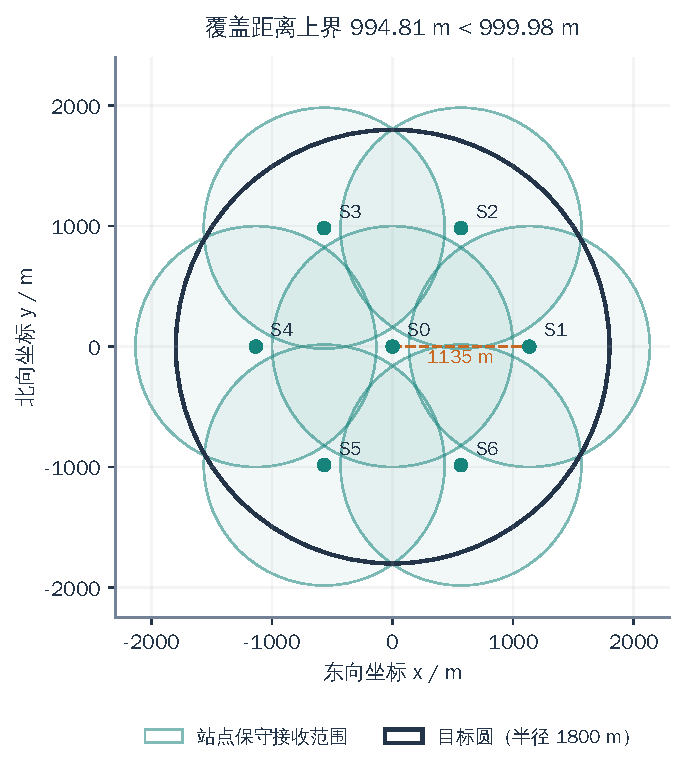
\includegraphics[width=0.67\textwidth]{F004-q3-coverage.pdf}
  \caption{全向源七站覆盖的几何证书；图中不表示实际运行轨迹}
  \label{fig:q3-coverage}
\end{figure}


\subsection{几何约束下的候选宏动作调度}
用公开请求与响应历史 $h_t$ 更新各频道的可行域、清除证书及覆盖进度，再生成候选集合 $\mathcal A(h_t)$。覆盖动作从最近的至多三个未访问站点中选择，串行检测未知频道及仍需补测的频道；已清除或已认证不存在的频道不再扫描。扫描优先使用当前频道，相邻站点交替频道顺序。

专门补测在可行域最小包围圆心的侧翼生成两个候选，方向垂直于最近示向度，偏移随包围圆半径限制在 $30$--$350\,\mathrm{m}$，每源至多专门补测三次。该实现使用问题二的交会几何思想，当前未调用其完整粗到细选点器。半径达到清除条件时前往包围圆心；返回近距离标志时优先原地清除。定位区域较小或补测次数达到阈值后，生成覆盖该区域的清除点序列，成功即停止。失败清除提供 $K_c\leftarrow K_c\setminus B(q,20)$ 的确定性信息。

候选包含覆盖、补测、保证清除、覆盖探测和退出五类宏动作。规则教师按估计成本排序，学习策略对同一集合评分，随后展开为串行请求。退出只在全部频道已清除或已认证不存在时开放；累计发现 $16$ 个不同频道后，可利用题面上界认证其余频道不存在。学习模块不能修改几何证书或放宽退出条件。

算法输入为公开历史 $h_t$ 与冻结参数，输出为一个合法宏动作。任务开始时，各频道均置为未知状态，机器人从题设初始位置生成首批覆盖候选；每执行一个宏动作便更新可行域和频道状态，再重新生成候选。若候选超出计算预算，则回退到规则教师；当全部频道取得清除或不存在证书时输出退出动作。这一接口把初始化、状态更新、回退与停止条件固定下来，参数化策略只改变候选的相对次序。

\begin{figure}[htbp]
\centering

\includegraphics[width=0.96\textwidth]{F001-controller-workflow.pdf}
\caption{在线控制器从公开历史更新证书、生成合法候选并执行后重新规划的闭环流程}
\end{figure}

\subsection{公开信息驱动的集合式候选评分}
覆盖结构决定哪些频道尚待搜索，几何证书决定哪些清除动作可靠，但两者并不唯一确定执行次序。为联合考虑信息获取和行动成本，将当前全局状态、各频道状态及候选动作分别编码。全局输入为 $10$ 维，频道输入为 $20\times9$ 维，每个候选为 $11$ 维，均由公开响应生成，真实源数与隐藏位置不输入策略。

频道编码经过两层四头注意力网络，隐藏维度为 $128$、前馈维度为 $256$，随后平均汇聚。候选编码与全局、频道汇聚编码拼接，输出动作分数 $\ell_\theta(h,a)$：
\begin{equation}
 \pi_\theta(a\mid h)=\frac{\exp\ell_\theta(h,a)}{\sum_{b\in\mathcal A(h)}\exp\ell_\theta(h,b)},\qquad a\in\mathcal A(h).
\end{equation}
变长候选以掩码处理；在线选择最高分宏动作，执行后重新生成候选。两问采用相同结构、分别冻结参数，每个网络含 $352386$ 个参数。频道聚合用于刻画待处理任务之间的联系，最终模型不包含候选与单频道之间的交叉注意力，也不包含粒子信念网络。

\subsection{以完整任务时间校准候选次序}
单独压缩移动路程可能推迟新源发现；只奖励成功清除又可能诱导过早停止。因此，将从任务开始到取得退出依据的全部虚拟时间纳入回报，采用
\begin{equation}
 r_t=-\frac{\Delta T_t}{100}-1000\mathbb I\{t\text{为失败终局}\},\qquad\gamma=1.
\end{equation}
其中失败终局包括未完成全部清除的回合。训练奖励不读取真实源数作归一化；逐局 $T/N$ 仅在评估与验证选模时计算。参数更新采用 PPO 剪切目标\cite{schulman2017}，记概率比为 $\rho_t=\pi_\theta(a_t\mid h_t)/\pi_{\rm old}(a_t\mid h_t)$，则策略项为
\begin{equation}
 \mathcal L_{\rm actor}=-\mathbb E\left[\min\left(\rho_t\widehat A_t,
 \operatorname{clip}(\rho_t,0.8,1.2)\widehat A_t\right)\right].
\end{equation}
优势估计采用 $\lambda=0.95$，并结合价值拟合与熵正则进行更新；每轮执行两个优化周期，近似 KL 超过 $0.03$ 时共同停止。训练时采样动作，部署时固定选择最高分动作。几何层始终独立维护合法候选及退出条件，策略无法通过提前退出换取较高回报。

方法的关键是把\textbf{发现覆盖、几何清除和不存在认证作为约束，把整局耗时作为调度目标}。PPO 是参数求解工具，其本身不作为本文原创算法；本文针对本题构造的覆盖证书、状态与动作接口共同限定了它的优化空间。前期相容场景搜索与数据聚合用于研究候选价值，相关实验保留在支撑材料，不将历史探索模块全部计入最终在线流程。

\subsection{完整性与独立实验结果}
在题设静态与有界误差条件下，七站覆盖保证每个存在的全向源至少可被一个站点检测；正观测持续更新保守可行域，必要时对该域构造有限清除覆盖。退出仅在 $20$ 个频道均已清除或已认证不存在时开放。因此，完整性来自覆盖与终止条件，不能用“连续若干次无信号”替代。

最终模型在 $3000$ 个独立研究场景中全部完成，共 $38961$ 个源全部发现并清除，\textbf{源级清除率与整局完成率均为 $100\%$}。含无源确认的平均总虚拟时间为 $3255.76\,\mathrm{s}$，逐局每源耗时的平均值为 $255.99\,\mathrm{s}/\text{源}$。相对同批父模型，平均总时间减少 $15.28\,\mathrm{s}$，每源耗时减少 $1.17\,\mathrm{s}$，配对区间见第九节。该结论是有限测试的实测表现，不把随机试验本身视为连续域完备性证明。

\subsection{正式测试记录的证据边界}
最终模型的上述结果来自自建研究环境。本次交付未提供问题三三次正式测试的完整成绩单，故不以研究结果填充正式成绩。提交时须由原始回放补齐案例编码、清除源数、平均定位清除时间及程序运行时间。

\section{问题四：定向干扰源下的模型扩展}

\subsection{定向状态扩维}
将发射模式 $m_i$ 和方向 $\phi_i$ 加入隐状态。对于无信号观测，似然函数同时考虑距离条件与方向覆盖条件，从而避免把所有无信号区域简单排除。

\subsection{稳健策略}
训练和评测阶段随机化目标位置、接收半径、发射方向与测向误差。若信念规划在规定步数内未完成任务，则启动确定性覆盖扫描，并在终止前逐频道复核。\placeholder{填写全向与定向混合场景的最终成绩。}

\section{模型检验与实验设计}

\subsection{规则实现与工程验证}
为避免在正式测试前反复消耗机会，依据题面和附件中的公开规则搭建独立本地模拟器，对物理转移、接口协议、客户端重试、计时、回放和调试网页进行验证。当前可复现结果如\cref{tab:engineering-validation}所示。

\begin{table}[H]
  \centering
  \caption{当前工程验证结果}
  \label{tab:engineering-validation}
  \begin{tabularx}{\textwidth}{LYL}
    \toprule
    验证项目 & 结果 & 适用范围 \\
    \midrule
    自动化回归测试 & 59 项及 69 个参数化子测试通过 & 几何、覆盖、协议、回放与策略接口 \\
    附件计时回放 & $0,105,111,194,199,199$ s & 与附件给定动作序列一致 \\
    参考内核与快速内核对比 & 10000 步无差异 & 固定本地夹具 \\
    距离阈值邻域检查 & 48 组无差异 & 本地数值边界样例 \\
    题面及两份附件校验 & 3 份通过 & 仓库保存的原始文件 \\
    \bottomrule
  \end{tabularx}
\end{table}

上述测试说明已列出的公开规则和确定性夹具可复现，不代表本地场景与官方隐藏随机机制同分布，也不能代替问题三、问题四的完整策略效果实验。

\subsection{自建研究分布上的配对实验}
在固定的 \texttt{LOCAL-RESEARCH/research-v1-20260911} 分布上，对问题三的四组独立配置分别完成 512 次 PPO 更新，并分别在 64 个未参与更新的场景上与确定性教师策略配对比较，共得到 $256$ 对留出结果。两种策略的完成率均为 $100\%$；确定性基线与学习策略的平均虚拟时间分别为 $3743.90\,\mathrm{s}$ 和 $3353.06\,\mathrm{s}$，平均配对差为 $-390.85\,\mathrm{s}$，相对下降 $10.44\%$。按独立场景近似计算，平均差的 $95\%$ 区间半宽为 $45.29\,\mathrm{s}$。学习策略的平均路程由 $15131.36\,\mathrm{m}$ 降至 $13136.99\,\mathrm{m}$，平均失败清除次数由 $7.10$ 降至 $3.41$，但平均检测次数由 $105.97$ 略增至 $109.30$。

问题四此前仅有 $8$ 个小样本配对场景；虽然平均差为 $-114.60\,\mathrm{s}$，其近似 $95\%$ 区间跨越零。最新大规模训练记录进一步显示，四组教师基线的完成率仅为 $10.94\%$--$21.09\%$；重启后的 PPO 训练进行到第 154--157 次更新时，留出完成率仍为 $14.06\%$--$18.75\%$。因此问题四当前结果暴露的是终止与退出逻辑缺陷，不能作为策略改进证据，论文仍以连续域覆盖证书和确定性兜底作为可信结论。

\begin{table}[H]
  \centering
  \caption{自建研究分布上的策略配对结果}
  \label{tab:research-paired}
  \begin{tabularx}{\textwidth}{cYLLLL}
    \toprule
    问题 & 场景数 & 基线完成率 & 策略完成率 & 平均时间差/s & 近似 $95\%$ 半宽/s \\
    \midrule
    三 & $256$ & $100\%$ & $100\%$ & $-390.85$ & $45.29$ \\
    四（初步） & $8$ & $100\%$ & $100\%$ & $-114.60$ & $315.97$ \\
    \bottomrule
  \end{tabularx}
\end{table}

\begin{figure}[H]
  \centering
  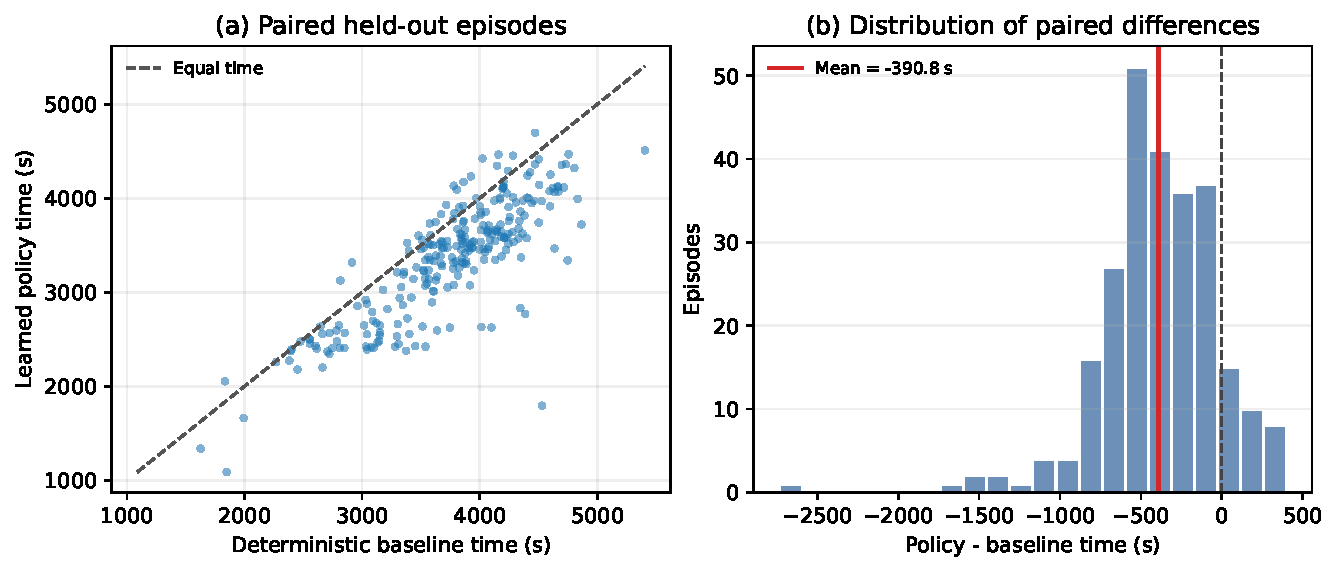
\includegraphics[width=0.94\textwidth]{q3_large_paired.pdf}
  \caption{问题三 256 个留出场景的配对时间比较；虚线表示两策略耗时相同，负差值表示学习策略更快}
  \label{fig:q3-large-paired}
\end{figure}

训练与评估均只使用公开历史构造的状态特征；非法动作在采样前屏蔽。问题三最终配对验证的原始记录、配置和来源信息已从远端协作分支提交 \texttt{4d75bee} 原样归档至 \texttt{results/validation/q3-large-4d75bee/}，汇总值由 256 条记录重新计算。另以其中一组最优权重进行 3000 个独立随机场景的稳定性压力测试，全部完成任务，共清除 39024 个源；逐场景计算的平均每源耗时为 $261.65\,\mathrm{s}$，按全部源加权为 $256.23\,\mathrm{s}$。该试验没有配对基线，只支持稳定性判断；原始记录归档于 \texttt{results/validation/q3-3000-9e10994/}。以上均为非官方研究分布结果，正式运行仍以完成率不低于确定性基线为首要选择条件。

\subsection{策略评价指标}
每局记录实际源数 $N$、成功清除数 $C$、清除比例 $C/N$、累计虚拟时间 $T$、平均定位清除时间 $T/C$、程序运行时间、总路程、检测次数、频道切换次数、失败清除次数和最大单步决策耗时。比较方案时对相同场景进行配对测试，同时报告均值、标准差和失败案例。

\subsection{对照与灵敏度分析}
问题三至少比较 $a=1130,1135,1140,1150\,\mathrm{m}$ 的六边形覆盖骨架，以及“发现后立即追踪”和“覆盖途中顺路定位”两种调度。问题四比较不同网格平移、旋转和边长；任何候选首先通过连续域覆盖检查，再比较站点数和路线长度。问题二改变 $\lambda_1$、粗候选数量和局部细化范围，考察最坏后验半径与总时间的权衡。\placeholder{补充问题二参数灵敏度图，以及问题三、四的完整轨迹与退出证书图；新增数据必须链接到固定代码版本及原始运行记录。}

\section{模型评价与推广}
\subsection{模型优点}
\begin{enumerate}
\item \textbf{完整性有明确的退出依据。}各频道必须已清除或已认证不存在；源数未知时仍完成无遗漏搜索，达到 $16$ 个不同源后才使用数量上限缩减覆盖。两问独立测试均实现 $3000/3000$ 完成和 $100\%$ 源级清除率。
\item \textbf{几何保证与效率估计分别核验。}接收、覆盖和清除条件由有界误差集合与几何证书给出，候选评分只改变动作次序；不会以估计概率代替不存在证明。
\item \textbf{行动成本采用一致的全程口径。}移动、检测、切换、处置及无源确认均计入虚拟时间。最后清除与合法退出分开统计，避免把确认开销遗漏后误判效率。
\item \textbf{结论可追溯到同一模型与样本。}最终模型主结果、父模型规划对照、有利布局和官方交互单例分别标注身份，防止将不同算法或不同终点的数值拼接比较。
\end{enumerate}

\subsection{模型局限}
固定站点提供充分覆盖条件，并未证明站点数或总路线最优。几何外包和数值保护量可能延迟清除；进一步细分非凸可行域有望降低保守性。问题二的有限情景评分没有连续全局最优保证，且其完整选点器尚未直接接入多源部署策略。

最终 Q4 相对父模型的配对区间跨零，延长参数优化尚未形成可确认的显著收益。完整无源确认产生的长尾更值得关注，但任何删点、提前终止或路线变更都需重新验证退出依据。主动搜索得到的最短/最长布局只反映已检验候选，不能作为全局极值。

全部大样本性能来自自建研究分布；有限样本的 $100\%$ 完成不等于跨任意分布的统计保证。理论发现证书亦不自动保证在任意现实计算预算内完成：通信中断、数值边界和动作预算仍需工程核验。已归档的官方单例使用父模型，最终两问各三次正式测试及全程序运行时间仍待原始成绩确认。

\subsection{模型推广}
该方法可推广到有界观测误差下的移动传感器搜索：将传感器可见范围转化为覆盖条件，以平台的真实动作成本替换虚拟时间，再对合法动作排序。遇到障碍物或移动目标时，应分别引入可达路径或动态可行域传播，并重新证明覆盖与清除条件。

\section{结论}
本文以\textbf{完整发现、全部清除和无遗漏退出}为先决条件，建立有界误差集合定位、保证接收选点和证书约束调度模型。问题一以可复现三角形反例说明直径不超过 $40$ m 并不足以保证清除；问题二的 $120$ 场景配对显示，稀疏候选平均节省 $5.74$ s，但平均后验半径增加 $3.68$ m，揭示局部精度与完整行动成本的权衡。

问题三以七站圆盘覆盖保证全向发现，问题四以 $31$ 站三角网格处理未知发射方向。最终模型在两问各 $3000$ 个独立研究场景中均全部完成，共清除 $38961$ 和 $39086$ 个源，\textbf{完整任务完成率和源级清除率均为 $100\%$}；含无遗漏确认的平均每源时间分别为 $255.99$ s 与 $767.25$ s。Q3 相对父模型的平均每源时间降低约 $0.453\%$；Q4 仅有小幅均值改善，配对区间跨零，未证明显著收益。

有利布局及规划对照表明，最后一个已发现源的清除时刻与完整搜索终点必须区分。$N<16$ 时未知频道仍需认证，发现数达到 $16$ 时才可利用数量上界停止其余覆盖。本文给出的最快构造样例用于解释这一完整性成本，并非所有策略的耗时下界。最终成绩仍须结合两问各三次正式测试记录核验。

% 使用2026配套样式中的官方声明句式；用途须按本队实际情况补全。
\CumcmAIUsed{资料检索、建模思路整理、代码调试、LaTeX排版和语言润色}
AI生成或修改的内容均由队员结合题面、程序输出与原始记录逐项核验；未取得的正式测试结果未由AI补写。具体使用过程、采纳内容与人工修改情况见支撑材料中的《AI工具使用详情》。

\begin{thebibliography}{99}
  \bibitem{pomdp}
  Kaelbling L P, Littman M L, Cassandra A R. Planning and acting in partially observable stochastic domains[J]. Artificial Intelligence, 1998, 101(1-2): 99-134.

  \bibitem{particle}
  Arulampalam M S, Maskell S, Gordon N, et al. A tutorial on particle filters for online nonlinear/non-Gaussian Bayesian tracking[J]. IEEE Transactions on Signal Processing, 2002, 50(2): 174-188.

  \bibitem{replace}
  \placeholder{补充正文实际引用的中文、英文文献，并删除本占位条目。}
\end{thebibliography}

\clearpage
\begin{appendices}
\section{支撑材料文件列表}
\begin{table}[H]
  \centering
  \caption{支撑材料文件列表}
  \begin{tabularx}{\textwidth}{LL}
    \toprule
    文件或目录 & 功能说明 \\
    \midrule
    \texttt{src/bsim/} & 本地模拟器、协议客户端、计时与回放工具 \\
    \texttt{src/solution/} & 几何、覆盖、主动选点、控制器和学习策略实现 \\
    \texttt{scripts/} & 参数构造、配对评估、覆盖核验和模型导出入口 \\
    \texttt{tests/} & 规则、协议、计时、几何边界和策略接口测试 \\
    \texttt{handoff/tables/} & 论文表格的原始数据、计算口径和来源记录 \\
    \texttt{handoff/figures/} & 论文插图的 PDF、PNG 与可编辑 SVG 文件 \\
    \texttt{runs/} & 参数配置、检查点、逐局记录和独立评估汇总 \\
    \texttt{results/} & 演练与正式测试记录的固定归档位置 \\
    \texttt{README.md}、\texttt{pyproject.toml} & 环境、依赖、命令和复现说明 \\
    《AI工具使用详情》 & AI工具用途、采纳内容与人工核验记录 \\
    \bottomrule
  \end{tabularx}
\end{table}
\section{核心程序与复现入口}
完整可运行源码随支撑材料一并提交。为便于核验，\cref{tab:reproduce-entry}列出本文各结论对应的程序入口；正式提交包中保留配置文件、随机种子、冻结检查点和逐局原始记录，使表图能够从同一版本重新生成。

\begin{table}[H]
  \centering
  \caption{模型实现与结果复现入口}
  \label{tab:reproduce-entry}
  \begin{tabularx}{\textwidth}{LL}
    \toprule
    程序入口 & 对应内容 \\
    \midrule
    \path{src/solution/geometry/core.py} & 角域求交、最远点对与最小包围圆 \\
    \path{src/solution/planning/q2.py} & 问题二保证接收约束与粗到细选点 \\
    \path{src/solution/coverage/certificates.py} & 全向七站与定向三角网格覆盖证书 \\
    \path{src/solution/control/controller.py} & 频道状态、合法候选、回退与退出控制 \\
    \path{src/solution/search/teacher.py} & 相容场景搜索、配对代价与标签筛选 \\
    \path{src/solution/rl/} & 候选评分、数据聚合与整局目标校准 \\
    \path{scripts/evaluate_3000.py} & 冻结策略的独立大样本评估 \\
    \path{scripts/validate_coverage.py} & 连续域覆盖条件和几何参数复核 \\
    \bottomrule
  \end{tabularx}
\end{table}

正式测试完成后，将原始响应、逐步动作、虚拟时间分解、程序运行时间和退出证书保存到 \path{results/formal/}，再由同一复算脚本生成问题三、四的正式结果表。
\end{appendices}

\end{document}
